\documentclass[11pt]{article}

\usepackage[a4paper,margin=1in]{geometry}
\usepackage{amsmath,amssymb,amsthm,mathtools}
\usepackage{booktabs,tabularx,array}
\usepackage{graphicx}
\usepackage{float}
\usepackage{microtype}
\usepackage{xcolor}
\usepackage{tikz}
\usetikzlibrary{arrows.meta,positioning,calc,fit,backgrounds}
\usepackage{hyperref}
\usepackage[nameinlink,noabbrev]{cleveref}

\hypersetup{
  colorlinks=true,
  linkcolor=blue!55!black,
  citecolor=green!40!black,
  urlcolor=blue!60!black,
  pdftitle={Fast and Reproducible Enumeration of 2 by C Sudoku Grids through C=5}
}

\newtheorem{theorem}{Theorem}[section]
\newtheorem{proposition}[theorem]{Proposition}
\newtheorem{lemma}[theorem]{Lemma}
\newtheorem{corollary}[theorem]{Corollary}
\theoremstyle{definition}
\newtheorem{definition}[theorem]{Definition}
\theoremstyle{remark}
\newtheorem{remark}[theorem]{Remark}

\newcommand{\Sym}{\mathcal{S}}
\newcommand{\PM}{\mathop{\mathrm{PM}}}
\newcommand{\Orb}{\mathop{\mathrm{Orb}}}
\newcommand{\Aut}{\mathop{\mathrm{Aut}}}
\newcommand{\comp}[1]{\overline{#1}}
\newcommand{\Nfive}{1\,903\,816\,047\,972\,624\,930\,994\,913\,280\,000}
\newcommand{\artifacturl}{https://github.com/ChopperLin/sudoku_FJ}

\title{Fast and Reproducible Enumeration of\\
       \texorpdfstring{$2\times C$}{2 by C} Sudoku Grids through
       \texorpdfstring{$C=5$}{C=5}}
\author{Author name(s) to be supplied before submission}
\date{Draft of July 12, 2026}

\begin{document}

\maketitle

\begin{abstract}
We give a self-contained exact enumeration method for completed
$2C\times2C$ Sudoku grids whose regions have shape $2\times C$.
Pettersen announced the $C=5$ count in 2005 and later published symmetry
data, but the historical pages we located do not provide a buildable
reproduction artifact.  We reformulate the historical band-class sum in
terms of balanced binary-pattern orbits and ordered one-factorizations of
regular bipartite graphs.  The resulting identity is
\[
  N(C)=\sum_{[h]}m(h)F_C(Q_h)^2,
\]
where $h$ ranges over signed-coordinate orbits of balanced pattern
histograms, $m(h)$ is an exact labelled multiplicity, and $F_C(Q_h)$ is the
number of ordered one-factorizations of a $C$-regular bipartite graph.
For $C=5$, this outer reduction replaces $252^5$ labelled skeletons by only
$355$ exact weighted terms.  Two rooted identities then make the inner count
small: a least-frequency edge-pivot recurrence for general degree and an
output-sensitive two-factor split that closes degree four directly at the
cycle base case.
An open C++20 implementation reproduces all known counts for $2\le C\le5$.
For $C=5$ it obtains
\[
  N(5)=\Nfive
\]
in a mean end-to-end time of $8.66$ seconds over five runs on an AMD Ryzen 9
9950X3D, with an observed peak working set of $66.1$ MiB.  A separate
transfer-kernel implementation in the same artifact reaches the same integer
through a different state space.  The paper is a reproducible verification
and algorithmic account; it does not claim priority for the numerical value.
\end{abstract}

\section{Introduction}

A completed $2\times C$ Sudoku is a $2C\times2C$ array on $2C$ symbols in
which every row, every column, and every $2\times C$ region contains each
symbol exactly once.  These arrays are rectangular-region Sudoku squares, a
special family of gerechte designs; see Bailey, Cameron, and
Connelly~\cite{bailey2008gerechte} for broader design-theoretic context.
Despite the elementary definition, exact enumeration becomes difficult
quickly.

Exact Sudoku enumerations have traditionally combined symmetry reduction
with exhaustive completion counts.  Felgenhauer and Jarvis used this strategy
for ordinary $9\times9$ Sudoku~\cite{felgenhauer2006enumerating}; Russell and
Jarvis then applied Burnside's lemma to count its symmetry classes
\cite{russell2006symmetry}.  The present work follows that
computational-combinatorial tradition for rectangular regions.

The known total counts through $C=5$ are recorded as OEIS
A291187~\cite{oeisA291187}.  The largest one was announced by Kjell Fredrik
Pettersen in an October 2005 forum post~\cite{pettersen2005c5}:
\[
  N(5)=\Nfive.
\]
That post reports roughly ten hours of computation and $355$ equivalence
classes of band configurations.  A later Jarvis-hosted page gives
Pettersen's Burnside table for the stronger problem of counting essentially
different grids~\cite{pettersen2008symmetry}.  After quotienting symbol
labels, its identity-class entry is
\[
  524\,640\,665\,777\,288\,616\,345\,600;
\]
multiplication by $10!$ recovers $N(5)$ exactly.

Pettersen also announced a $C=6$ total in 2006, based on $63\,199$ outer
classes~\cite{pettersen2006c6}:
\[
  N(6)=38\,296\,278\,920\,738\,107\,863\,746\,324\,732\,012\,492\,486\,187\,417\,600\,000.
\]
We do not verify that much larger computation here.  This historical source
matters for priority: $C=6$ is an outstanding
\emph{independent-verification} target, not an unpublished numerical target.

The public historical pages provide the numerical result, class counts, and
an outline of the decomposition, but we located no linked buildable source
artifact for the $C=5$ computation.  The purpose of the present work is to
make the calculation mathematically explicit and routinely reproducible.
Our contributions are as follows.

\begin{itemize}
  \item We express a band configuration as a balanced histogram on the
        Boolean cube and give its exact labelled multiplicity under signed
        coordinate permutations.  At $C=5$ this reduces $252^5$ labelled
        skeletons to $355$ exact orbit records.
  \item We identify the completion count of one stack with the number of
        ordered one-factorizations of a regular bipartite graph.  This gives
        a short proof of the historical outer sum.
  \item We use a rooted perfect-matching recurrence and prove a specialized
        degree-four two-factor identity.  Together with exact bipartite graph
        canonization, these reduce the top-level matching workload by a
        factor of $5.10$ and bypass the entire cubic residual layer.
  \item We provide source code, build scripts, exact gates for $C=2,3,4,5$,
        and a second algorithmic route in the public artifact
        \cite{artifact2026}.
\end{itemize}

The proof and the acceleration separate cleanly.  The orbit--factorization
identity accounts for every labelled grid; the rooted identities change only
how each exact $F_C(Q_h)$ is evaluated.  The full reduction is shown in
\cref{fig:pipeline}, while \cref{fig:inner-shortcuts} isolates the two inner
shortcuts.  Both diagrams are part of the LaTeX source.

\begin{figure}[t]
  \centering
  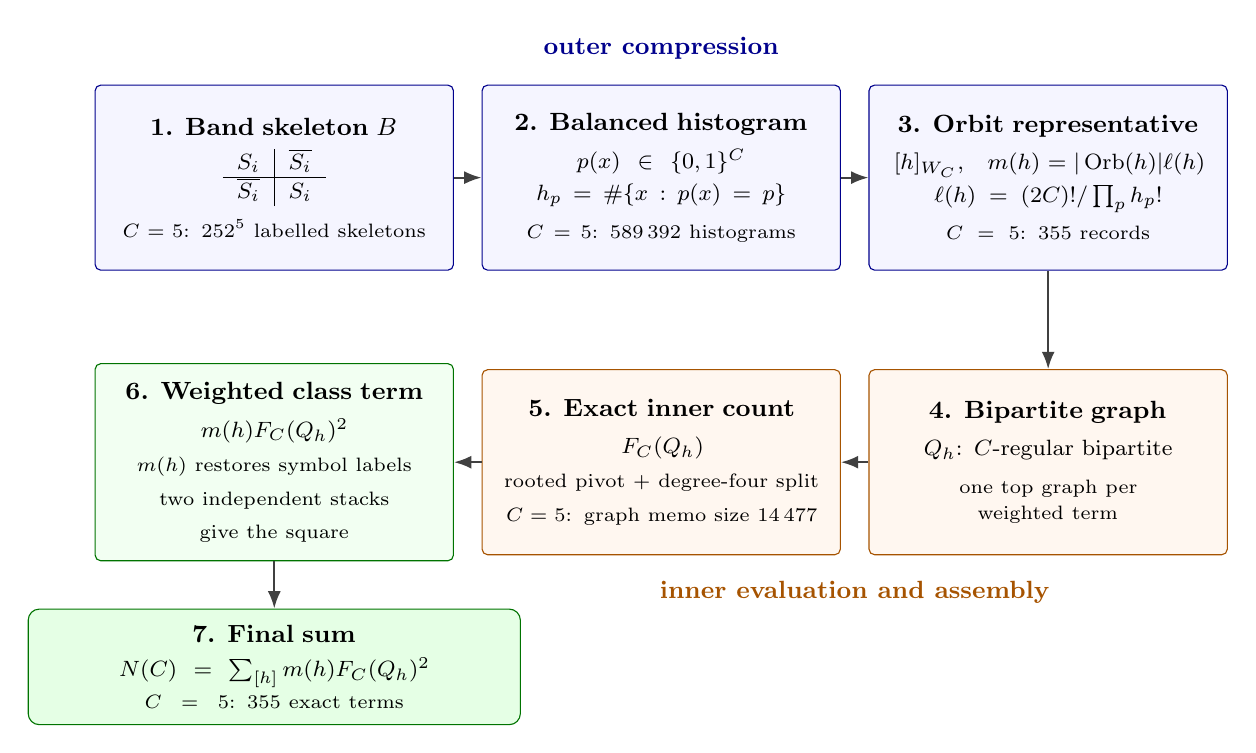
\begin{tikzpicture}[
      font=\footnotesize,
      stage/.style={rounded corners=2pt,text width=4.05cm,
        minimum height=2.35cm,align=center,inner xsep=2.5mm,inner ysep=2.4mm},
      outerstage/.style={stage,draw=blue!55!black,fill=blue!4},
      innerstage/.style={stage,draw=orange!65!black,fill=orange!6},
      sumstage/.style={stage,draw=green!45!black,fill=green!5},
      totalstage/.style={draw=green!45!black,fill=green!10,rounded corners,
        text width=5.75cm,minimum height=1.35cm,align=center,
        inner xsep=2.5mm,inner ysep=2mm},
      arrow/.style={-{Latex[length=2.2mm]},thick,draw=black!75}
    ]
    \node[outerstage] (skeleton) {
      {\small\bfseries 1. Band skeleton $B$}\\[1.4mm]
      $\begin{array}{c|c}S_i&\comp{S_i}\\ \hline
      \comp{S_i}&S_i\end{array}$\\[1.4mm]
      {\scriptsize $C=5$: $252^5$ labelled skeletons}};
    \node[outerstage,right=0.35cm of skeleton] (hist) {
      {\small\bfseries 2. Balanced histogram}\\[1.4mm]
      $p(x)\in\{0,1\}^C$\\[0.8mm]
      $h_p=\#\{x:p(x)=p\}$\\[1.4mm]
      {\scriptsize $C=5$: $589\,392$ histograms}};
    \node[outerstage,right=0.35cm of hist] (orbit) {
      {\small\bfseries 3. Orbit representative}\\[1.4mm]
      $[h]_{W_C}$,\quad $m(h)=|\Orb(h)|\ell(h)$\\[0.8mm]
      $\ell(h)=(2C)!/\prod_p h_p!$\\[1.4mm]
      {\scriptsize $C=5$: $355$ records}};

    \node[innerstage,below=1.25cm of orbit] (graph) {
      {\small\bfseries 4. Bipartite graph}\\[1.4mm]
      $Q_h$: $C$-regular bipartite\\[1.4mm]
      {\scriptsize one top graph per weighted term}};
    \node[innerstage,left=0.35cm of graph] (fact) {
      {\small\bfseries 5. Exact inner count}\\[1.4mm]
      $F_C(Q_h)$\\[1.0mm]
      {\scriptsize rooted pivot $+$ degree-four split}\\[1.0mm]
      {\scriptsize $C=5$: graph memo size $14\,477$}};
    \node[sumstage,left=0.35cm of fact] (term) {
      {\small\bfseries 6. Weighted class term}\\[1.4mm]
      $m(h)F_C(Q_h)^2$\\[1.0mm]
      {\scriptsize $m(h)$ restores symbol labels}\\[1.0mm]
      {\scriptsize two independent stacks}\\[0.8mm]
      {\scriptsize give the square}};
    \node[totalstage,below=0.60cm of term] (total) {
      {\small\bfseries 7. Final sum}\\[1.0mm]
      $N(C)=\sum_{[h]}m(h)F_C(Q_h)^2$\\[0.8mm]
      {\scriptsize $C=5$: $355$ exact terms}};

    \node[above=2mm of hist,font=\small\bfseries,text=blue!55!black]
      {outer compression};
    \node[below=2mm of $(fact.south)!0.5!(graph.south)$,
      font=\small\bfseries,text=orange!65!black]
      {inner evaluation and assembly};

    \draw[arrow] (skeleton.east) -- (hist.west);
    \draw[arrow] (hist.east) -- (orbit.west);
    \draw[arrow] (orbit.south) -- (graph.north);
    \draw[arrow] (graph.west) -- (fact.east);
    \draw[arrow] (fact.west) -- (term.east);
    \draw[arrow] (term.south) -- (total.north);
  \end{tikzpicture}
  \caption{The complete enumeration pipeline, with the exact $C=5$ workload
  shown at each compression stage.  The orbit record supplies both a graph
  representative and its labelled multiplicity.  The vertical arrow
  enters $Q_h$ directly: graph construction precedes, and is distinct from,
  the inner one-factorization count.}
  \label{fig:pipeline}
\end{figure}

\section{Skeletons and regular bipartite graphs}
\label{sec:skeleton}

Let $X$ be a set of $2C$ symbols.  Index the bands by $i\in[C]$, the two rows
inside a band by $\varepsilon\in\{0,1\}$, the two stacks by
$s\in\{0,1\}$, and the $C$ columns inside a stack by $j\in[C]$.

\begin{definition}[Band skeleton]
For each band $i$, let $S_i\subset X$ be the set of symbols appearing in row
$(i,0)$ inside stack $0$.  The ordered sequence
$B=(S_1,\ldots,S_C)$ is the \emph{skeleton} of the grid.
\end{definition}

\begin{lemma}[Forced complements]
Each $S_i$ has size $C$, and the four row--stack symbol sets in band $i$ are
\[
\begin{array}{c|cc}
 & s=0 & s=1\\ \hline
\varepsilon=0 & S_i & \comp{S_i}\\
\varepsilon=1 & \comp{S_i} & S_i.
\end{array}
\]
\end{lemma}

\begin{proof}
Each $2\times C$ region contains all $2C$ symbols, so the two rows inside a
region contain complementary $C$-subsets.  Each complete row also contains
all symbols, so its subsets in the two stacks are complementary.  Starting
from $S_i$ forces the other three entries in the table.
\end{proof}

Represent the skeleton by a binary matrix
$B=(b_{i,x})\in\{0,1\}^{C\times2C}$, where $b_{i,x}=1$ exactly when
$x\in S_i$.  Every row of $B$ has weight $C$.

From $B$ construct a bipartite graph $Q_B$ with left vertex set
\[
  L=[C]\times\{0,1\}
\]
and right vertex set $X$.  Join $(i,0)$ to $x$ when $b_{i,x}=1$, and join
$(i,1)$ to $x$ otherwise.  Every left vertex has degree $C$.  For each
$i$, a symbol $x$ is adjacent to exactly one of $(i,0)$ and $(i,1)$, so every
right vertex also has degree $C$.  Thus $Q_B$ is a $C$-regular bipartite
graph with $2C$ vertices on each side.

\begin{definition}[Ordered one-factorization count]
For a $d$-regular bipartite graph $G$, let $F_d(G)$ be the number of ordered
tuples $(M_1,\ldots,M_d)$ of pairwise edge-disjoint perfect matchings whose
union is $E(G)$.
\end{definition}

\begin{proposition}[One-stack bijection]
For a fixed skeleton $B$, the number of legal fillings of stack $0$ is
$F_C(Q_B)$.
\end{proposition}

\begin{proof}
An edge $((i,\varepsilon),x)$ records the occurrence of symbol $x$ in the
corresponding row of stack $0$.  Assign the edge color $j$ when that occurrence
is placed in the $j$th column of the stack.  Every row uses each of the $C$
columns once exactly when all colors occur once at every left vertex.  Every
full column uses each symbol once exactly when all colors occur once at every
right vertex.  Hence each color class is a perfect matching, and the $C$
labeled columns give an ordered one-factorization.  Reversing the construction
recovers the unique stack filling.
\end{proof}

The graph for stack $1$ is obtained from $Q_B$ by swapping $(i,0)$ and
$(i,1)$ for every $i$.  It is therefore isomorphic to $Q_B$.  Once the
skeleton is fixed, the within-stack assignments are independent.

\begin{corollary}
The number of completed grids with skeleton $B$ is $F_C(Q_B)^2$.
\label{cor:square}
\end{corollary}

\section{Boolean-cube histograms and the outer orbit sum}
\label{sec:outer}

For each symbol $x\in X$, define its membership pattern
\[
  p(x)=(b_{1,x},\ldots,b_{C,x})\in\{0,1\}^C.
\]
After forgetting symbol names, the skeleton is determined by the histogram
\[
  h_p=\#\{x\in X:p(x)=p\},\qquad p\in\{0,1\}^C.
\]
The row-weight constraints become
\begin{equation}
  \sum_{p}h_p=2C,
  \qquad
  \sum_{p:p_i=1}h_p=C\quad(i\in[C]).
  \label{eq:balance}
\end{equation}
Call a nonnegative integer histogram satisfying \eqref{eq:balance}
\emph{balanced}.

Permuting bands permutes the coordinates of $p$.  Swapping the two rows in
band $i$ complements coordinate $i$.  These operations generate the signed
coordinate group
\[
  W_C=(\mathbb Z/2\mathbb Z)^C\rtimes\Sym_C,
  \qquad |W_C|=2^C C!.
\]
They act on balanced histograms and induce bipartite graph isomorphisms, so
$F_C(Q_h)$ is constant on every $W_C$-orbit.

For a balanced histogram $h$, the number of ways to assign the $2C$ symbol
labels to its pattern cells is
\[
  \ell(h)=\frac{(2C)!}{\prod_{p\in\{0,1\}^C}h_p!}.
\]
Let $o(h)=|\Orb_{W_C}(h)|=|W_C|/|\operatorname{Stab}_{W_C}(h)|$ and define
\begin{equation}
  m(h)=o(h)\ell(h).
  \label{eq:multiplicity}
\end{equation}

\begin{theorem}[Orbit--factorization identity]
Let $\mathcal H_C$ be a set of representatives of the $W_C$-orbits of
balanced histograms.  Then
\begin{equation}
  \boxed{
  N(C)=\sum_{h\in\mathcal H_C}m(h)F_C(Q_h)^2.}
  \label{eq:master}
\end{equation}
\end{theorem}

\begin{proof}
There are $\binom{2C}{C}^C$ labeled skeletons, since each of the $C$ bands
chooses one $C$-subset.  Within a fixed histogram orbit, there are $o(h)$
distinct histograms and $\ell(h)$ labeled skeletons for each histogram.
Thus \eqref{eq:multiplicity} is exactly the number of labeled skeletons in
that class.  Distinct histogram orbits are disjoint and exhaustive.  By
\cref{cor:square}, every labeled skeleton represented by $h$ contributes
$F_C(Q_h)^2$ completed grids.  Summing gives \eqref{eq:master}.
\end{proof}

The implementation enumerates every balanced histogram for $C\le5$, traverses
its orbit using coordinate flips and adjacent coordinate swaps, and retains
one canonical representative.  Stabilizers and multiplicities are computed
exactly.  The independent mass check is
\begin{equation}
  \sum_{h\in\mathcal H_C}m(h)=\binom{2C}{C}^{C}.
  \label{eq:masscheck}
\end{equation}
The observed outer counts are shown in \cref{tab:outer}.  For $C=6$, where
direct balanced-histogram generation is too large, the artifact instead uses
coordinate-by-coordinate canonical augmentation; it independently obtains
the historical $63\,199$ outer classes, but the full inner sum is outside the
scope of this paper.

\begin{table}[H]
  \centering
  \caption{Exact outer enumeration.  The last column is checked by
  \eqref{eq:masscheck}, not assumed.}
  \label{tab:outer}
  \begin{tabular}{rrrr}
    \toprule
    $C$ & balanced histograms & $W_C$-orbits & $\sum_h m(h)$ \\
    \midrule
    2 & 3       & 2   & $36=6^2$ \\
    3 & 28      & 4   & $8\,000=20^3$ \\
    4 & 1\,450  & 26  & $24\,010\,000=70^4$ \\
    5 & 589\,392& 355 & $1\,016\,255\,020\,032=252^5$ \\
    \bottomrule
  \end{tabular}
\end{table}

\section{Counting ordered one-factorizations}
\label{sec:factor}

The direct recurrence for a $d$-regular bipartite graph is
\begin{equation}
  F_d(G)=\sum_{M\in\PM(G)}F_{d-1}(G-M),
  \qquad F_1(G)=1.
  \label{eq:plainrec}
\end{equation}
We share memoized residual-graph values across all outer classes, modulo
independent permutations of the two bipartition sides.  Two elementary rooted
identities provide most of the speedup.  They act at different levels:
rooting reduces the number of residuals created, whereas the degree-four
identity removes a whole recursive layer.  Their roles are summarized in
\cref{fig:inner-shortcuts}.

\begin{figure}[H]
  \centering
  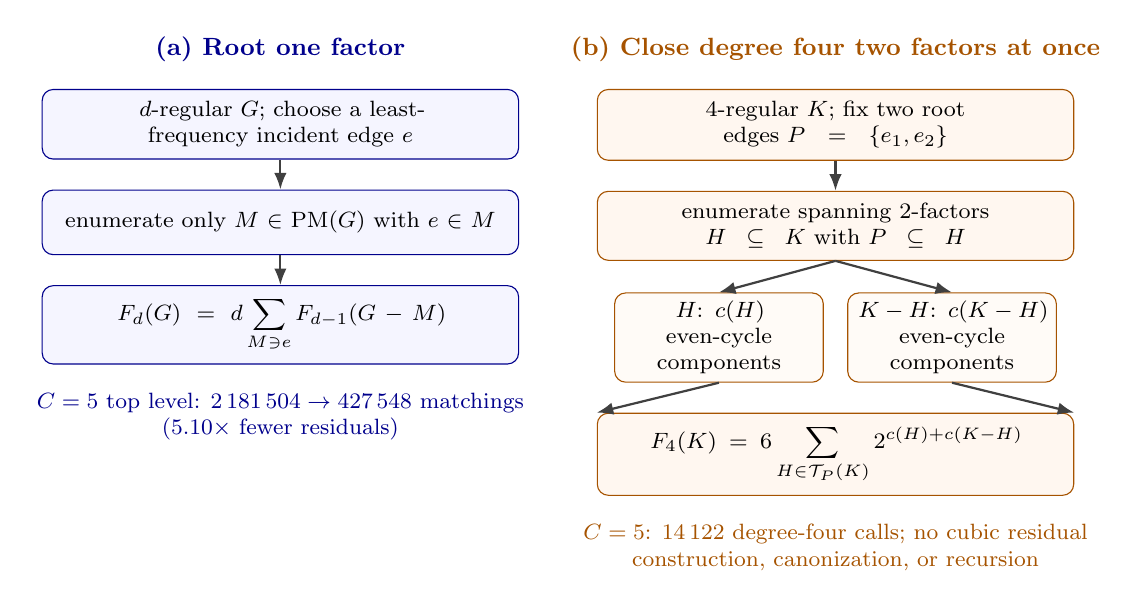
\begin{tikzpicture}[
      font=\footnotesize,
      pivotbox/.style={draw=blue!55!black,fill=blue!4,rounded corners,
        text width=5.75cm,minimum height=0.82cm,align=center,inner sep=1.5mm},
      splitbox/.style={draw=orange!65!black,fill=orange!6,rounded corners,
        text width=5.75cm,minimum height=0.82cm,align=center,inner sep=1.5mm},
      cyclebox/.style={draw=orange!65!black,fill=orange!3,rounded corners,
        text width=2.45cm,minimum height=0.74cm,align=center,inner sep=1mm},
      arrow/.style={-{Latex[length=2.1mm]},thick,draw=black!75}
    ]
    \node[font=\small\bfseries,text=blue!55!black] (ltitle) at (0,0)
      {(a) Root one factor};
    \node[pivotbox,below=0.22cm of ltitle] (lg)
      {$d$-regular $G$; choose a least-frequency incident edge $e$};
    \node[pivotbox,below=0.38cm of lg] (lm)
      {enumerate only $M\in\PM(G)$ with $e\in M$};
    \node[pivotbox,below=0.38cm of lm] (lf)
      {$F_d(G)=d\displaystyle\sum_{M\ni e}F_{d-1}(G-M)$};
    \node[below=0.24cm of lf,align=center,text=blue!55!black] (lstat)
      {$C=5$ top level: $2\,181\,504\to427\,548$ matchings\\
       ($5.10\times$ fewer residuals)};
    \draw[arrow] (lg.south) -- (lm.north);
    \draw[arrow] (lm.south) -- (lf.north);

    \node[font=\small\bfseries,text=orange!65!black] (rtitle) at (7.05,0)
      {(b) Close degree four two factors at once};
    \node[splitbox,below=0.22cm of rtitle] (rg)
      {$4$-regular $K$; fix two root edges $P=\{e_1,e_2\}$};
    \node[splitbox,below=0.38cm of rg] (rh)
      {enumerate spanning $2$-factors $H\subseteq K$ with $P\subseteq H$};
    \node[cyclebox,below=0.40cm of rh.south,xshift=-1.48cm] (rhc)
      {$H$: $c(H)$\\even-cycle components};
    \node[cyclebox,below=0.40cm of rh.south,xshift=1.48cm] (rcc)
      {$K-H$: $c(K-H)$\\even-cycle components};
    \node[splitbox,below=0.38cm of $(rhc.south)!0.5!(rcc.south)$] (rf)
      {$F_4(K)=6\displaystyle\sum_{H\in\mathcal T_P(K)}2^{c(H)+c(K-H)}$};
    \node[below=0.24cm of rf,align=center,text=orange!65!black] (rstat)
      {$C=5$: $14\,122$ degree-four calls; no cubic residual\\
       construction, canonization, or recursion};
    \draw[arrow] (rg.south) -- (rh.north);
    \draw[arrow] (rh.south) -- (rhc.north);
    \draw[arrow] (rh.south) -- (rcc.north);
    \draw[arrow] (rhc.south) -- (rf.north west);
    \draw[arrow] (rcc.south) -- (rf.north east);
  \end{tikzpicture}
  \caption{The two inner shortcuts.  The edge pivot is a one-colour
  restriction with an exact multiplicative correction.  At degree four, the
  root pair identifies two factor labels; their union and its complement are
  both unions of even cycles, so the count closes directly through
  \eqref{eq:f2}.  The workload annotations are from the full $C=5$ run.}
  \label{fig:inner-shortcuts}
\end{figure}

The distinction is important.  The pivot is a branching reduction and is
valid at every degree.  The two-factor split is stronger but special to
degree four: it turns the cycle formula from a base case into a direct
closure.  The controlled ablation in \cref{tab:ablation} measures both effects
separately.

\subsection{Rooted edge pivot}

\begin{proposition}[Rooted recurrence]
Fix any edge $e\in E(G)$ of a $d$-regular bipartite graph.  Then
\begin{equation}
  F_d(G)=d\sum_{\substack{M\in\PM(G)\\e\in M}}F_{d-1}(G-M).
  \label{eq:rooted}
\end{equation}
\end{proposition}

\begin{proof}
In every ordered one-factorization, exactly one of the $d$ factors contains
$e$.  Remove that factor and retain the order of the other $d-1$ factors.
Conversely, a matching $M\ni e$ and an ordered factorization of $G-M$ yield
$d$ ordered factorizations of $G$, according to the position at which $M$ is
inserted.
\end{proof}

For a fixed left vertex $u$, the frequencies
\[
  f(uv)=\#\{M\in\PM(G):uv\in M\}
\]
sum to $|\PM(G)|$ over the $d$ edges incident with $u$.  A subset dynamic
program on the other left vertices computes all $f(uv)$ exactly in
$O((2C)2^{2C})$ arithmetic operations.  We choose the least frequent incident
edge as the root.  At $C=5$, aggregated over the $355$ top graphs, this reduces
the perfect matchings passed to the recurrence from $2\,181\,504$ to
$427\,548$, a factor of $5.10$.

\subsection{The degree-two base case}

A $2$-regular bipartite graph is a disjoint union of even cycles.  Each cycle
has two alternating perfect matchings, and choices on distinct cycles are
independent.  Therefore
\begin{equation}
  F_2(G)=2^{c(G)},
  \label{eq:f2}
\end{equation}
where $c(G)$ is the number of connected components.

\subsection{A rooted two-factor split at degree four}

Let $G$ be $4$-regular, fix a left vertex $u$, and fix two distinct edges
$P=\{e_1,e_2\}$ incident with $u$.  Let $\mathcal T_P(G)$ be the set of
spanning $2$-factors $H\subseteq G$ that contain both edges of $P$.

\begin{proposition}[Degree-four split]
\begin{equation}
  F_4(G)=6\sum_{H\in\mathcal T_P(G)}2^{c(H)+c(G-H)}.
  \label{eq:rooted4}
\end{equation}
\end{proposition}

\begin{proof}
For a fixed $H$, equation \eqref{eq:f2} gives $2^{c(H)}$ ordered ways to
split $H$ into two perfect matchings, and $2^{c(G-H)}$ ordered ways to split
the complement.  Choose which two of the four global factor labels belong to
$H$ in $\binom42=6$ ways.

Conversely, in any ordered four-factorization the two root edges in $P$ have
two distinct factor labels.  The union of precisely those two factors is the
unique member $H\in\mathcal T_P(G)$ associated with that factorization.
Thus every ordered factorization is counted exactly once on the right-hand
side.
\end{proof}

\begin{remark}[Why the split is decisive]
The identity is more than a faster way to enumerate the first matching.
Ordinary recursion would construct, canonicalize, and memoize cubic graphs
before eventually reaching degree two.  Equation~\eqref{eq:rooted4} instead
groups the four factor labels into the unique pair selected by $P$ and its
complement, then evaluates both pieces immediately by their cycle counts.
The factor $6=\binom42$ restores the choice of the selected label pair, so no
symmetry assumption about $G$ is involved.
\end{remark}

The implementation enumerates $\mathcal T_P(G)$ without constructing cubic
residual graphs.  It processes the left vertices one at a time and selects two
incident edges for $H$.  A ternary state records the current degree
$0,1,$ or $2$ of every right vertex.  A forward reachability pass over at most
$3^{2C}$ states identifies viable predecessors.  A backward, output-sensitive
pass then emits only completed $2$-factors.  Two rollback disjoint-set data
structures maintain $c(H)$ and $c(G-H)$, so each leaf contributes the exact
weight in \eqref{eq:rooted4}.

\subsection{Exact residual-graph memoization}

Residual graphs are canonicalized under independent permutations of their
left and right vertices.  The canonicalizer uses equitable refinement and
individualization, following the standard refinement--individualization
paradigm~\cite{mckay2014practical}.  A configurable search budget cannot
affect correctness.  If a search exceeds the budget, the program stores a
weaker key consisting of the complete adjacency matrix after sorting left
rows, in a namespace disjoint from canonical keys.  Equal weak keys represent
identical labeled graphs up to a left-row permutation; unequal weak keys may
miss an isomorphic merge but can never merge nonisomorphic graphs.  Hence a
fallback costs only time and memory.  The reported $C=5$ run encountered two
such safe fallbacks.

\section{Correctness of the complete algorithm}

The correctness argument has three separately checkable layers.  First, the
forced-complement and one-stack bijections turn completed grids into labelled
skeletons weighted by $F_C(Q_B)^2$.  Second, the Boolean-cube orbit partition
groups those skeletons without changing their total multiplicity.  Third, the
rooted identities evaluate each $F_C(Q_h)$ exactly; canonicalization and
memoization only reuse already equal values.  The next theorem composes these
layers and makes explicit that none of the performance heuristics is an
assumption in the count.

\begin{theorem}
For every $2\le C\le5$, the algorithm implemented by
\texttt{factorization\_orbit.cpp} returns the exact number $N(C)$ of completed
$2\times C$ Sudoku grids.
\end{theorem}

\begin{proof}
The forced-complement lemma gives a unique skeleton for every completed grid.
The one-stack bijection and \cref{cor:square} give the exact number of grids
above each skeleton.  The histogram orbit partition is exhaustive and
disjoint, and \eqref{eq:multiplicity} counts its labeled skeletons exactly;
hence \eqref{eq:master} is exact.

For every graph in \eqref{eq:master}, equations \eqref{eq:rooted},
\eqref{eq:f2}, and \eqref{eq:rooted4} are exact counting identities.
Canonical graph keys merge only isomorphic residual graphs, while a budget
fallback can only decline a merge.  Memoization therefore changes neither an
individual factorization count nor the outer sum.  All arithmetic is unsigned
exact integer arithmetic.  For $C\le5$, every positive intermediate is at most
the final total $N(5)<2^{128}$, so the 128-bit representation is sufficient.
\end{proof}

\section{Implementation and reproducibility}
\label{sec:repro}

The reference implementation is C++20 and has no third-party run-time
dependency.  It is available at
\begin{center}
  \url{\artifacturl}.
\end{center}
The measurements below use source commit
\texttt{d86cd88383da915e33caf8e361cfb193134953dc}; the SHA-256 digest of
\texttt{src/factorization\_orbit.cpp} is
\begin{center}
\texttt{A19A951E613E5305A1E8A4E34A9CF5CC52FF76FF7B512819D5D7103E67691EA8}.
\end{center}
From the repository root on Windows, the exact build and run are
\begin{verbatim}
powershell -NoProfile -ExecutionPolicy Bypass -File scripts\build_og2.ps1
.\build\factorization_orbit.exe 5 pivot rooted4
\end{verbatim}
The underlying compilation command is
\begin{verbatim}
g++ -O3 -mpopcnt -fopenmp -std=c++20 -I src \
    src/factorization_orbit.cpp -o build/factorization_orbit.exe
\end{verbatim}
The executable prints the outer mass check, the final integer, detailed
operation counters, and an explicit \texttt{[OK]} comparison with the known
decimal value.  No checkpoint or precomputed table is used for $C=5$.

The benchmark platform was Windows 11 Pro 64-bit (build 26100), MinGW-w64 GCC
13.2.0, and an AMD Ryzen 9 9950X3D with 16 physical cores and 32 logical
processors.  The machine has 128 GiB of RAM.  Only batched graph canonization
uses OpenMP; the outer enumeration and principal recursive control flow are
serial.

\section{Results and validation}
\label{sec:results}

\Cref{tab:counts} reports a fresh run made after rebuilding the artifact from
the pinned source.  ``Factor'' is the time for all graph counts and the exact
sum, while ``outer'' is the time for balanced-histogram orbit enumeration.

\begin{table}[H]
  \centering
  \caption{Exact counts and measured running times on the benchmark platform.
  Times below a millisecond are included only as regression information.}
  \label{tab:counts}
  \begin{tabular}{r>{\raggedleft\arraybackslash}p{8.0cm}rr}
    \toprule
    $C$ & $N(C)$ & factor (s) & outer (s) \\
    \midrule
    2 & $288$ & 0.0004 & 0.0002 \\
    3 & $28\,200\,960$ & 0.0009 & 0.0002 \\
    4 & $29\,136\,487\,207\,403\,520$ & 0.0086 & 0.0008 \\
    5 & $\Nfive$ & 7.7934 & 0.8087 \\
    \bottomrule
  \end{tabular}
\end{table}

\subsection{Controlled algorithmic ablation}

To isolate the contribution of the two rooted identities, we rebuilt the
pinned source once and ran four consecutive clean processes.  Every row used
the same executable, graph canonicalizer, and outer enumeration, and every row
reproduced the exact $C=5$ integer with an explicit \texttt{[OK]}.  Only the
two named algorithm flags changed.

\begin{table}[H]
  \centering
  \caption{Controlled $C=5$ ablation on the benchmark platform.  Factor time
  excludes the common outer enumeration.  ``Canon.'' counts exact
  canonicalization computations, not cache lookups.}
  \label{tab:ablation}
  \small
  \begin{tabular}{lrrrrr}
    \toprule
    inner method & factor (s) & speedup & matchings & graph calls & canon. \\
    \midrule
    plain recurrence
      & 53.35 & $1.00\times$ & $14\,191\,134$ & $5\,820\,174$ & $7\,933\,335$ \\
    edge pivot only
      & 36.93 & $1.44\times$ & $3\,256\,904$ & $1\,999\,603$ & $2\,471\,437$ \\
    degree-four split only
      & 11.48 & $4.65\times$ & $2\,181\,504$ & $357\,320$ & $1\,426\,850$ \\
    edge pivot $+$ degree-four split
      &  8.58 & $6.22\times$ & $427\,548$ & $119\,959$ & $320\,221$ \\
    \bottomrule
  \end{tabular}
\end{table}

The ablation identifies the principal gain.  The degree-four identity removes
the cubic residual layer and cuts recursive graph calls by more than an order
of magnitude.  The edge pivot then composes with that shortcut: aggregated
over the $355$ top graphs, it retains $427\,548$ of $2\,181\,504$ perfect
matchings.  The final run evaluates $40\,488\,962$ rooted two-factor leaves,
but each leaf needs only two rollback updates and a cycle-weight addition; it
does not create or canonicalize another graph.

The first working graph-factorization prototype took $254.996$ seconds on the
same machine.  That figure is useful development history but is not a
controlled speedup baseline, because later versions also improved data
structures and canonicalization.  By contrast, every row of
\cref{tab:ablation} comes from the same current binary.

\subsection{Timing stability and thread sensitivity}

Five additional clean-process $C=5$ runs with the default 32 OpenMP threads
had end-to-end times
\[
  8.64,\ 8.70,\ 8.67,\ 8.64,\ 8.66\ \text{seconds},
\]
with mean $8.66$ seconds.  A 20-ms polling monitor observed a peak working set
of $66.1$ MiB in every run.  Single observations with fixed OpenMP thread
counts are shown in \cref{tab:threads}; the modest scaling is expected because
only canonicalization batches are parallel.

\begin{table}[H]
  \centering
  \caption{$C=5$ thread-count sensitivity.  Wall time includes process startup.}
  \label{tab:threads}
  \begin{tabular}{rrrr}
    \toprule
    OpenMP threads & factor (s) & outer (s) & wall (s) \\
    \midrule
    1  & 13.527 & 0.810 & 14.445 \\
    8  &  8.221 & 0.780 &  9.044 \\
    16 &  7.892 & 0.788 &  8.729 \\
    32 &  7.837 & 0.824 &  8.709 \\
    \bottomrule
  \end{tabular}
\end{table}

\subsection{Workload compression and independent checks}

The $C=5$ run generated $589\,392$ balanced histograms and reduced them to
$355$ outer orbits.  Its multiplicities summed to
$252^5=1\,016\,255\,020\,032$.  The inner stage stored $14\,477$ exact graph
values, made $119\,959$ graph calls with $105\,482$ memo hits, enumerated
$427\,548$ rooted perfect matchings, and evaluated $14\,122$ degree-four
graphs using \eqref{eq:rooted4}.  Every structural check and final decimal
comparison passed.

Correctness is not based solely on agreement with the last integer.
The artifact contains the following additional checks.

\begin{enumerate}
  \item The same program reproduces $C=2,3,4$ before $C=5$.
  \item The outer multiplicity identity \eqref{eq:masscheck} is checked for
        every $C$.
  \item Canonization invariance, separation, and histogram differential tests
        are run against slower reference routines.
  \item A separate quotient transfer-kernel program, \texttt{multiset\_q.cpp},
        obtained the same $C=5$ integer after $5.45$ active hours with a peak
        resident set of approximately $16.33$ GiB.  It evolves anonymous
        column-mask multisets band by band and does not call the
        orbit--factorization engine.
  \item The result agrees both with Pettersen's 2005 decimal and prime
        factorization~\cite{pettersen2005c5}, and with the identity entry of
        the later symmetry table after multiplication by $10!$
        \cite{pettersen2008symmetry}.
\end{enumerate}

Comparing directly with the approximately ten-hour 2005 computation would
mix algorithmic improvement with two decades of hardware progress.  We
therefore report it only as historical context and use \cref{tab:ablation},
not the historical runtime, for quantitative speedup claims.

\section{Scope, limitations, and outlook}

This paper verifies the total labeled count A291187(5).  It does not recompute
Pettersen's full Burnside table or the essentially different count
$4\,743\,933\,602\,050\,718$ recorded as A291188.  Doing so would require
fixed-point counts for nontrivial Sudoku symmetries, not merely the identity
term handled here.

The method extends formally to $C=6$, and its outer augmentation reproduces
the historical count of $63\,199$ skeleton classes.  The inner distribution is
far less favorable: low-symmetry outer graphs produce tens of thousands of
nonisomorphic degree-five residuals.  A full independent verification of
Pettersen's announced $C=6$ integer remains future work.  In particular, the
seconds-scale $C=5$ result should not be extrapolated as evidence for a
seconds- or hours-scale $C=6$ computation.

Several nearer extensions are concrete.  First, the $355$ weighted outer
terms can be published as a compact machine-checkable certificate rather than
only regenerated from source.  Second, an independent implementation of the
rooted degree-four identity would strengthen the software-level audit.
Third, adapting the factorization formulation to symmetry-fixed grids could
independently verify A291188(5), the headline result of Pettersen's Burnside
calculation.

\section*{Acknowledgments}

The historical computations of Kjell Fredrik Pettersen, Ed Russell, Bertram
Felgenhauer, and Frazer Jarvis made the target values and decomposition ideas
available to the community.  This draft deliberately separates their
priority for the counts from the reproducibility and algorithmic contributions
of the present work.

\bibliographystyle{alpha}
\bibliography{references}

\appendix

\section{Minimal reproducibility checklist}

Starting from a clean checkout of the pinned source commit:
\begin{enumerate}
  \item build with \texttt{scripts/build\_og2.ps1};
  \item run \texttt{scripts/verify\_og2.ps1};
  \item run \texttt{factorization\_orbit.exe 5 pivot rooted4};
  \item verify both printed lines
\begin{verbatim}
outer multiplicity sum=1016255020032 expected=1016255020032 [OK]
expected=1903816047972624930994913280000 [OK]
\end{verbatim}
\end{enumerate}
The larger repository verification script
\texttt{scripts/verify\_all.ps1} additionally rebuilds every
active engine, repeats the $C=2,3,4,5$ factorization gates, reproduces the
classical $9\times9$ count through two routes, and checks the preserved
read-only $C=6$ checkpoint when it is locally available.

\end{document}
